\documentclass[a4paper,onecolumn]{article}

\usepackage{graphicx}          % För att få grafik att fungera.
\usepackage{amsmath}           % Innehåller vissa matematiska symboler.
\usepackage[utf8]{inputenc}  % Ser till så att svenska tecken fungerar. Om du sparar filen i UTF-8, byt latin1 mot utf8.
\usepackage[english]{babel}    % LaTeX tänker svenskt.
\usepackage{url}	       % För att ange URL:er


                               
\usepackage{cite}
\usepackage{tabularx}
\usepackage{siunitx}
\usepackage[a4paper, total={6in, 8in}]{geometry}

\usepackage{bigfoot} % to allow verbatim in footnote
\usepackage[numbered,framed]{matlab-prettifier}
\usepackage{filecontents}

\usepackage[parfill]{parskip} % No newline indentation

\usepackage{url}
\usepackage{float}
\usepackage{subfig}
\usepackage{bm}
\usepackage{tikz}
\usepackage{physics}
\usepackage{courier}
\usepackage[font=small,labelfont = small]{caption}


\usepackage{pythonhighlight}

\usepackage{listings}
\usepackage{color}

\usepackage{fancyvrb}
\usepackage{fancyvrb}
\usepackage{fvextra}
\usepackage{xcolor}

% Utseende
\addtolength{\topmargin}{10mm}% Drar bort 20mm från övre marginalen kommentera bort raden om du är nöjd med avståndet. Det finns fler parametrar att justera om du inte får plats på det utsatta antalet sidor.
\addtolength{\textheight}{10mm}% Det vi drog bort från topmargin lägger vi till i texthöjden.
\geometry{left=20mm,right=20mm,top=20mm, bottom=20mm}

% Code Color Scheme
\definecolor{code_black}{HTML}{282C34}
\definecolor{code_red}{HTML}{FF0000}
\definecolor{code_green}{HTML}{008000}
\definecolor{code_yellow}{HTML}{FFD800}
\definecolor{code_blue}{HTML}{1560BD}
\definecolor{code_magenta}{HTML}{FF33CC}
\definecolor{code_cyan}{HTML}{00BFFF}
\definecolor{code_white}{HTML}{A9A9A9}


\begin{document}



\title{COTS RDMA Data-Transfer}
\title{%
  COTS RDMA Data-Transfer \\
  \large Two throughput demos using UCX and Verbs}



\author{Isac Bruce, Hannes Ekstam Ljusegren}

\date{\today}


\maketitle



\section{Introduction}
A proposed method for writing and reading to a remote memory region is tested with real and synthetic data to measure speed of transfer. The programs utilizes the high performance networking library UCX to establish a communication layer between the endpoints or infinband Verbs. Furthermore, our demos was tested on two Dell Precision Workstations (Back-to-Back) running Ubuntu 20.04 LTS on Intel Xeon Processors using Mellanox ConnectX-6 Dx and Nvidia Quadro M4000 GPU's.

\subsection{Dictionary}
\begin{itemize}
   \item RDMA is Remote Direct Memory Access
   \item SmartNIC/HCA is the Smart Network interface card
 \end{itemize}

\begin{figure}[H]
\begin{center}
\subfloat[]{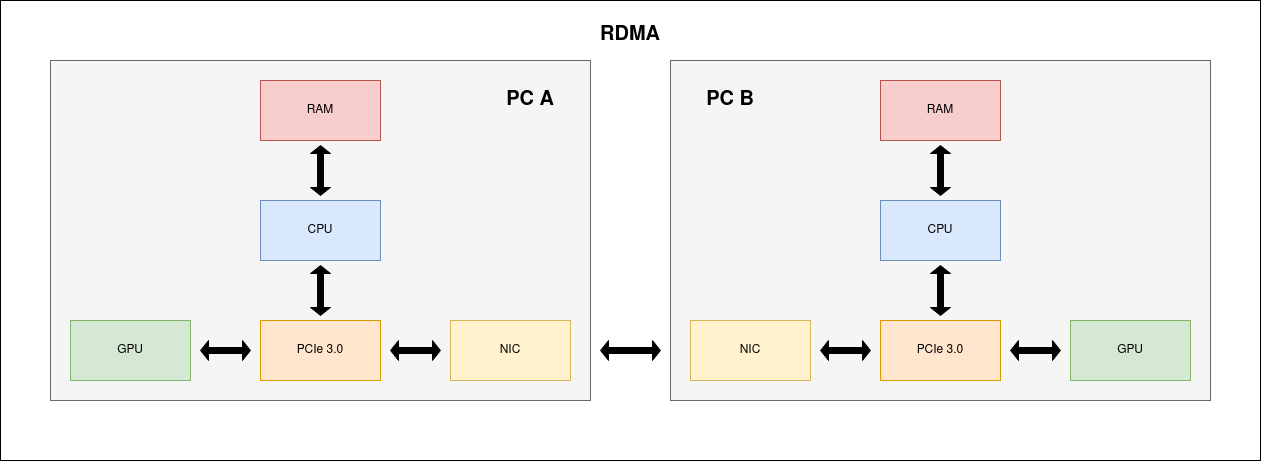
\includegraphics[width = 1\columnwidth]{rdma.png}}
\caption{Flowchart of RDMA for two computers connected with infiniband.}
\label{cpu-cpu-demo}
\end{center}
\end{figure}



\section{Setup}
In order to run the tests in the demo the following hardware and software requirements must be met:
\subsection{Hardware Requirements}
The following HCA's are high-performance 4X+ InfiniBand Host Channel Adapter
(HCA) cards that enable performance of high-speed (20+ Gbps) InfiniBand fabrics, with latency as low as 1.3 microseconds. 
\begin{itemize}
   \item ConnectX-6 Lx
   \item ConnectX-6 Dx  \textit{(Ours)}
   \item ConnectX-6
   \item ConnectX-5
   \item ConnectX-4 Lx
 \end{itemize}


Appropriate GPU's for RDMA data-transfer must be accessible by the host and the HCA. The following Nvidia GPU's have been confirmed by either Nvidia or peers TODO to support GPUDirect RDMA. TODO
AMD devices have not been tested or confirmed working using this method.

\begin{itemize}
   \item Tesla™ \textit{(any)}
   \item Quadro™ K-Series
   \item Quadro™ P-Series
   \item Quadro™ M-Series \textit{(Ours)}
 \end{itemize}

\subsection{Software Requirements}
In order to use the network interface cards, the package NVIDIA Firmware Tools: \verb|mft| must be installed for firmware management together with correct drivers for Linux \verb|MLNX_OFED|. 

In order to utilize GPUDirect RDMA, the package \verb|nvidia-peer-mem| must be installed.

To be able to control the host channel adapter (HCA), the HPC networking library \verb|ucx| is required with support for GPUDirect RDMA TODO.

\section{Installation}

\subsection{NVIDIA Drivers}
It is preffered to install display drivers using the distribution's native package management tool, i.e \verb|apt|. If not installed already, NVIDIA display drivers can be installed from NVIDIA Download Center, see: \url{https://www.nvidia.com/Download/index.aspx?lang=en-us.}

\subsection{CUDA Runtime and Toolkit}
To install CUDA Toolkit (CUDA 11.7) from Nvidia on Ubuntu 20.04:

\begin{Verbatim}[breaklines=true, breakanywhere=true, breaksymbol=, breakanywheresymbolpre=, commandchars=\\\{\}]
wget https://developer.download.nvidia.com/compute/cuda/repos/ubuntu2004/x86_64/cuda-ubuntu2004.pin
sudo mv cuda-ubuntu2004.pin /etc/apt/preferences.d/cuda-repository-pin-600
wget https://developer.download.nvidia.com/compute/cuda/11.7.0/local_installers/cuda-repo-ubuntu2004-11-7-local_11.7.0-515.43.04-1_amd64.deb

sudo dpkg -i cuda-repo-ubuntu2004-11-7-local_11.7.0-515.43.04-1_amd64.deb
sudo cp /var/cuda-repo-ubuntu2004-11-7-local/cuda-*-keyring.gpg /usr/share/keyrings/

sudo apt-get update
sudo apt-get -y install cuda
\end{Verbatim}

\subsection{Mellanox OFED}
Compatible versions for NIC firmware are v2.1-x.x.x or later. To install Linux drivers for ethernet
and infiniband adapters, \verb|MLNX_OFED|. See: Download Center \url{https://network.nvidia.com/products/infiniband-drivers/linux/mlnx\_ofed/ or for Ubuntu 20.04}:

\begin{Verbatim}[breaklines=true, breakanywhere=true, breaksymbol=, breakanywheresymbolpre=]
wget http://www.mellanox.com/downloads/ofed/MLNX_OFED-5.6-2.0.9.0/MLNX_OFED_LINUX-5.6-2.0.9.0-ubuntu20.04-x86_64.tgz
tar -xvf MLNX_OFED_LINUX*

cd MLNX_OFED_LINUX*
sudo ./mlnxofedinstall --upstream-libs --dpdk --force

sudo /etc/init.d/openibd restart
\end{Verbatim}

\subsection{GPUDirect RDMA}

To enable GPUDirect RDMA the Nvidia kernel module \verb|nvidia-peer-mem| must be installed. The module will be referred to as \verb|nvidia-peer-mem| and \verb|nv_peer_mem| interchangeably. To install \verb|nv_peer_mem| for Ubuntu 20.04 LTS:

\begin{Verbatim}[breaklines=true, breakanywhere=true, breaksymbol=, breakanywheresymbolpre=]
git clone https://github.com/Mellanox/nv_peer_memory.git
cd nv_peer_memory
./build_module.sh

cd /tmp
tar xzf /tmp/nvidia-peer-memory_*
cd nvidia-peer-memory-*
dpkg-buildpackage -us -uc
sudo dpkg -i /tmp/nvidia-peer-memory_*.deb

sudo service nv_peer_mem restart
\end{Verbatim}

*Note that this kernel module is deprecated and may not be supported in future releases.

\subsection{UCX}

To install \verb|ucx| on Ubuntu 20.04, python bindings are required together with python3+ packages. To maintain a working environment, installing \verb|conda| is highly recommended. 

\subsubsection{Conda}

\begin{enumerate}
    \item Installing on system:
\begin{Verbatim}[breaklines=true, breakanywhere=true, breaksymbol=, breakanywheresymbolpre=]
wget https://repo.anaconda.com/miniconda/Miniconda3-latest-Linux-x86.sh

bash Miniconda3-latest-Linux-x86.sh
\end{Verbatim}

    \item Disable auto-init \textit{(optional)}

\begin{verbatim}
conda config --set auto_activate_base false
\end{verbatim}

    \item Recreate an environment inside \verb|data-transfer|

\begin{verbatim}
conda env create -f environment.yml
\end{verbatim}

    \item Activate and enter the newly created environment
    
\begin{verbatim}
conda activate data-transfer
\end{verbatim}

\end{enumerate}

The terminal should now look like this:
\begin{Verbatim}[commandchars=\\\{\}]
\textcolor{code_green}{user@host}:\textcolor{code_blue}{~/data-transfer}$ conda activate data-transfer
(data-transfer) \textcolor{code_green}{user@host}:\textcolor{code_blue}{~/data-transfer}$
\end{Verbatim}

\subsubsection{Dependencies}

To build the project requires having some other modules not included in the conda environment:

\begin{verbatim}
pip install pynvml cpython
\end{verbatim}

\subsubsection{Development packages}

Ensure that the latest updates are installed by issuing the command \verb|sudo apt update -y|. Install the development packages \verb|libnuma-dev, cython3|. Using \verb|apt|:

\begin{verbatim}
sudo apt install -y libnuma-dev cython3
\end{verbatim}

\subsection{USB AC-68 Wi-Fi Adapter}
During the installation process, ASUS USB-AC68 Wireless-AC1900 Wi-Fi adapters were used for internet access. To install the network drivers for this dongle on Ubuntu 20.04, go to HTTPS://github.com/morrownr/8814au and follow the steps in the README.

*Note that secure boot was disabled during this project, as secure boot conflicted with the installation of the usb dongle. \\
*Note that you may need to install Linux modules extra if not already \\
\begin{verbatim}
$sudo apt-get install linux-modules-extra-$(uname -r)
\end{verbatim}

\section{Configuration}

\subsection{Networking}
The adapters need assigned IP addresses, we used the \verb|GNOME Network Manager| GUI and assigned the IPv4 addresses 10.0.0.x format with netmask 255.255.255.0

To run the demo, make sure both network adapters are connected and working properly by performing a ping. It is important to specify the correct interface when pinging:

\begin{verbatim}
ping -I <LOCAL_INTERFACE> <REMOTE_ADDRESS>
\end{verbatim}

Eg.:
\begin{Verbatim}[commandchars=\\\{\}]
(data-transfer) \textcolor{code_green}{user@scarecrow}:\textcolor{code_blue}{~/data-transfer}$ ping -I ens4f0np0 10.0.0.4
PING 10.0.0.4 (10.0.0.4) from 10.0.0.3 ens4f0np0: 56(84) bytes of data.
64 bytes from 10.0.0.4: icmp_seq=1 ttl=64 time=0.110 ms
64 bytes from 10.0.0.4: icmp_seq=2 ttl=64 time=0.112 ms
64 bytes from 10.0.0.4: icmp_seq=3 ttl=64 time=0.109 ms
^C
--- 10.0.0.4 ping statistics ---
3 packets transmitted, 3 received, 0% packet loss, time 2029ms
rtt min/avg/max/mdev = 0.109/0.110/0.112/0.001 ms
\end{Verbatim}

\pagebreak
To find which interface to ping, one could use \verb|ifconfig|:

\begin{Verbatim}[commandchars=\\\{\}]
(data-transfer) \textcolor{code_green}{user@scarecrow}:\textcolor{code_blue}{~/data-transfer}$ ifconfig

    eno1: flags=4099<UP,BROADCAST,MULTICAST>  mtu 1500
        ether 54:bf:64:6a:91:31  txqueuelen 1000  (Ethernet)
        RX packets 0  bytes 0 (0.0 B)
        RX errors 0  dropped 0  overruns 0  frame 0
        TX packets 0  bytes 0 (0.0 B)
        TX errors 0  dropped 0 overruns 0  carrier 0  collisions 0
        device interrupt 16  memory 0x92f00000-92f20000  

    # The one we used: Mellanox ConnectX-6 Dx (first port)
    -----------------
 -> \textcolor{code_red}{ens4f0np0}: flags=4163<UP,BROADCAST,RUNNING,MULTICAST>  mtu 1500
            inet \textcolor{code_red}{10.0.0.3}  netmask 255.255.255.0  broadcast 10.0.0.255
            inet6 fe80::4e4d:abee:c38d:4b6f  prefixlen 64  scopeid 0x20<link>
            ether 10:70:fd:60:c1:cc  txqueuelen 1000  (Ethernet)
            RX packets 1021  bytes 63776 (63.7 KB)
            RX errors 0  dropped 0  overruns 0  frame 0
            TX packets 841  bytes 52495 (52.4 KB)
            TX errors 0  dropped 0 overruns 0  carrier 0  collisions 0
    -----------------

    ens4f1np1: flags=4163<UP,BROADCAST,RUNNING,MULTICAST>  mtu 1500
            inet 10.0.0.1  netmask 255.255.255.0  broadcast 10.0.0.255
            inet6 fe80::40ba:65b6:cb4e:4521  prefixlen 64  scopeid 0x20<link>
            ether 10:70:fd:60:c1:cd  txqueuelen 1000  (Ethernet)
            RX packets 36  bytes 4419 (4.4 KB)
            RX errors 0  dropped 0  overruns 0  frame 0
            TX packets 23  bytes 3072 (3.0 KB)
            TX errors 0  dropped 0 overruns 0  carrier 0  collisions 0

    lo: flags=73<UP,LOOPBACK,RUNNING>  mtu 65536
            inet 127.0.0.1  netmask 255.0.0.0
            inet6 ::1  prefixlen 128  scopeid 0x10<host>
            loop  txqueuelen 1000  (Local Loopback)
            RX packets 1782  bytes 168796 (168.7 KB)
            RX errors 0  dropped 0  overruns 0  frame 0
            TX packets 1782  bytes 168796 (168.7 KB)
            TX errors 0  dropped 0 overruns 0  carrier 0  collisions 0

    wlx04421a4d9e71: flags=4163<UP,BROADCAST,RUNNING,MULTICAST>  mtu 1500
            inet 81.236.101.159  netmask 255.255.254.0  broadcast 81.236.101.255
            inet6 fe80::7207:baa6:6cea:6bd3  prefixlen 64  scopeid 0x20<link>
            ether 04:42:1a:4d:9e:71  txqueuelen 1000  (Ethernet)
            RX packets 66840  bytes 48821412 (48.8 MB)
            RX errors 0  dropped 7  overruns 0  frame 0
            TX packets 61150  bytes 44974817 (44.9 MB)
            TX errors 0  dropped 0 overruns 0  carrier 0  collisions 0
\end{Verbatim}

If the connection is working, building can be started.








\pagebreak
\section{Building and Usage}
To build the project, separate makefiles are provided for each demo. 

Building the UCX program will create 5 executable files: \verb|run, web_gauge, fpga_emulator, transfer_real| and \verb|transfer_synthetic|

Building the VERBS RDMA program will create 2 executable files: \verb|rdma_server| and \verb|rdma_client|
\vspace{5mm} %5mm vertical space

To build the programs, issue the \verb|make| command in the desired directory

Running the demo requires that both computers are connected via \verb|infiniband| and correct (see installation) software and modules are installed and running. 

To reproduce the demos, see documentation for each program.

\subsection{UCX}
All executables can be be configured with optional parameters (see \verb|--help|)


\subsubsection{fpga\_emulator}
\verb|fpga_emulator| is a program to emulate an incoming data-stream (data generator) to send from one GPU to the other combined with \verb|transfer_real|.

\subsubsection{web\_gauge}
\verb|web_gauge| is a web server displaying current transfer-speed in the style of a speedometer. The program receives current transfer-speed as double sent in a UDP package to the program in a specified port and address.

\subsubsection{transfer\_real}
\verb|transfer_real| is a demo utilizing incoming data from a socket, eg. a real device or \verb|fpga_emulator| and displays the bandwidth to \verb|web_gauge|.

\subsubsection{transfer\_synthetic}
\verb|transfer_synthetic| showcases the maximum inter transfer-speed between two nodes, ie. the program creates an array of ones, default is $\bm{2}^{26}$ bytes and writes to a remote region as fast as possible until the user interupts the program by \verb|<Ctrl-C>|. The program \verb|web_gauge| is also used to display the results.

\subsubsection{run}
\verb|run| is an experimental program utilizing CUDA code over a Cython-C-Cuda bridge known as \verb|cubridge.so| which is being built when building the demo. This can be used to call CUDA functions directly from Python code during runtime.

\subsection{Verbs RDMA}
This program clocks a CPU to remote GPU RDMA transfer.
The \verb|rdma_server| executable starts the server / sender with optional parameters (see -h), by default listening on port 20886 and IP of the NIC. The \verb|rdma_client| executable starts the client / receiver. The client takes an IP address and port number to connect to.

The client and server establishes a connection, shares a memory address of where to perform the RDMA, then proceeds to write 41943040000 bytes, in 2MB chunks. A custom handshake is performed to know when the receiver has successfully handled the sent(written) memory and the sender can begin the next transfer.













\section{Problems and Known Issues}

\subsection{Network Cards Shutting Down}

If the network adapters stops working after a period of time can be a result of insufficient cooling. The ConnectX cards require continuous cooling, we found that after exceeding 110°C, the modules were being unloaded from the system \verb|mlx5_core| followed by many warnings when shown with \verb|dmesg|. After exceeding the 120°C mark, the cards were physically shutdown by an onboard safety mechanism resulting in reloading the kernel modules was impossible and required a complete restart of the system. This happened without any load on the cards, around 2 minutes after a cold boot.

According to Nvidia \cite{article_nvidia_thermal_sensors}:

"The adapter card incorporates the ConnectX IC which operates in the range of temperatures between 0C and 105C.

There are three thermal threshold definitions which impact the overall system operation state:
\begin{itemize}
\item \textbf{Warning} – 105°C: On managed systems only: When the device crosses the 100°C threshold, a Warning Threshold message will be issued by the management SW, indicating to system administration that the card has crossed the Warning threshold. Note that this temperature threshold does not require nor lead to any action by hardware (such as adapter card shutdown).
 
\item \textbf{Critical} – 115°C: When the device crosses this temperature, the firmware will automatically shut down the device.

\item \textbf{Emergency} – 130°C: In case the firmware fails to shut down the device upon crossing the Critical threshold, the device will auto-shutdown upon crossing the Emergency (130°C) threshold.
\end{itemize}

The card's thermal sensors can be read through the system’s SMBus. The user can read these thermal sensors and adapt the system airflow in accordance with the readouts and the needs of the above-mentioned IC thermal requirements."

To check the current temperature of the installed cards, the command \verb|mget_temp| included in \verb|mft| can be used.

\vspace{5mm} %5mm vertical space
To find which card (location) to probe on the PCIe bus:

\begin{Verbatim}[commandchars=\\\{\}]
(data-transfer) \textcolor{code_green}{user@scarecrow}:\textcolor{code_blue}{~/data-transfer}$ lspci | grep Mellanox
\textcolor{code_magenta}{04:00.0} Ethernet controller: \textcolor{code_red}{Mellanox} Technologies MT2892 Family [ConnectX-6 Dx]
04:00.1 Ethernet controller: \textcolor{code_red}{Mellanox} Technologies MT2892 Family [ConnectX-6 Dx]
\end{Verbatim}

\vspace{5mm} %5mm vertical space
To probe \verb|04:00.0| (requires root privileges):

\begin{Verbatim}[commandchars=\\\{\}]
(data-transfer) \textcolor{code_green}{user@scarecrow}:\textcolor{code_blue}{~/data-transfer}$ sudo mget_temp -d 04:00.0
53
\end{Verbatim}


\subsection{Runtime Errors and Solutions}

\subsubsection{Aborted (core dumped) and UCX ERROR failed to register address/bad address}

If during runtime the following error occurs a solution is to use smaller buffers. We are not entirely sure how this issue is emerging. We found that a buffer size greater than \textcolor{code_magenta}{$>115MB$} would result in the following errors:

\begin{Verbatim}[commandchars=\\\{\}, breaklines=true, breakanywhere=true, breaksymbol=, breakanywheresymbolpre=]
(data-transfer) \textcolor{code_green}{user@scarecrow}:\textcolor{code_blue}{~/data-transfer}$ ./transfer_synthetic --transmitter -p 12377 -sp 45004 -a 10.0.0.4  --n-bytes \textcolor{code_magenta}{1000000000}
[1658921155.651848] [scarecrow:15571:0]          ib_log.c:254  \textcolor{code_red}{UCX  ERROR ibv_reg_mr(address=0x7fe574000000, length=1000000000, access=0xf) failed: Bad address}
[1658921155.651869] [scarecrow:15571:0]          ucp_mm.c:159  \textcolor{code_red}{UCX  ERROR failed to register address 0x7fe574000000 mem_type bit 0x2 length 1000000000 on md[3]=mlx5_0: Input/output error (md reg_mem_types 0x3)}
[1658921155.651874] [scarecrow:15571:0]     ucp_request.c:519  UCX  ERROR failed to register user buffer datatype 0x8 address 0x7fe574000000 len 1000000000: Input/output error
[scarecrow:15571:0:15571]        rndv.c:2378 Assertion `status == UCS_OK' failed
==== backtrace (tid:  15571) ====
0  /home/scarecrow/miniconda3/envs/data-transfer/lib/python3.7/site-packages/ucp/_libs/../../../../libucs.so.0(ucs_handle_error+0x2dc) [0x7fe71a27d7cc]
...
30  /home/scarecrow/miniconda3/envs/data-transfer/lib/libpython3.7m.so.1.0(+0x64416) [0x7fe71e8e0416]
31  /home/scarecrow/miniconda3/envs/data-transfer/lib/libpython3.7m.so.1.0(_PyEval_EvalFrameDefault+0x47a6) [0x7fe71e8e4f46]
36  ./transfer_synthetic(+0x10188) [0x55c38831d188]
37  ./transfer_synthetic(+0xae26) [0x55c388317e26]
38  /home/scarecrow/miniconda3/envs/data-transfer/lib/libpython3.7m.so.1.0(PyModule_ExecDef+0x4b)[0x7fe71ea2b3eb]
39  ./transfer_synthetic(+0xb709) [0x55c388318709]
40  ./transfer_synthetic(+0xbdaf) [0x55c388318daf]
41  /lib/x86_64-linux-gnu/libc.so.6(__libc_start_main+0xf3) [0x7fe71e6ae083]
42  ./transfer_synthetic(+0xbe91) [0x55c388318e91]
=================================
\textcolor{code_red}{Aborted (core dumped)}
\end{Verbatim}

\verb|BAR1| memory usage could be a part of the problem as BAR1 is used with RDMA transfer. To find out how much memory is accessible. Issue the command:

BAR1 Memory Usage

\begin{Verbatim}[commandchars=\\\{\}, breaklines=true, breakanywhere=true, breaksymbol=, breakanywheresymbolpre=]
(data-transfer) \textcolor{code_green}{user@scarecrow}:\textcolor{code_blue}{~/data-transfer}$ nvidia-smi -q
==============NVSMI LOG==============

Timestamp                                 : Fri Aug 12 12:58:30 2022
Driver Version                            : 515.65.01
CUDA Version                              : 11.7

Attached GPUs                             : 1
GPU 00000000:65:00.0
    Product Name                          : Quadro P4000
    Product Brand                         : Quadro
    Product Architecture                  : Pascal
...
    PCI
        Bus                               : 0x65
        Device                            : 0x00
        Domain                            : 0x0000
        Device Id                         : 0x1BB110DE
        Bus Id                            : 00000000:65:00.0
        Sub System Id                     : 0x11A31028
        GPU Link Info
            PCIe Generation
                Max                       : 3
                Current                   : 1
            Link Width
                Max                       : 16x
                Current                   : 16x
        Bridge Chip
            Type                          : N/A
            Firmware                      : N/A
        Replays Since Reset               : 0
        Replay Number Rollovers           : 0
        Tx Throughput                     : 0 KB/s
        Rx Throughput                     : 1000 KB/s
    Fan Speed                             : 46 %
    Performance State                     : P8
    Clocks Throttle Reasons
        Idle                              : Active
        Applications Clocks Setting       : Not Active
        SW Power Cap                      : Not Active
        HW Slowdown                       : Not Active
            HW Thermal Slowdown           : Not Active
            HW Power Brake Slowdown       : Not Active
        Sync Boost                        : Not Active
        SW Thermal Slowdown               : Not Active
        Display Clock Setting             : Not Active
    FB Memory Usage
        Total                             : 8192 MiB
        Reserved                          : 81 MiB
        Used                              : 482 MiB
        Free                              : 7628 MiB
\textcolor{code_red}{BAR1 Memory Usage  <-- 
        Total                             : 256 MiB
        Used                              : 15 MiB
        Free                              : 241 MiB}
    Compute Mode                          : Default
    Utilization
        Gpu                               : 11 %
        Memory                            : 14 %
        Encoder                           : 0 %
        Decoder                           : 0 %
...
\end{Verbatim}

\subsection{ucp.\_libs.exceptions.UCXError: Device is busy}

Current port is busy, terminate the process using it or use another port

\subsection{UCX  WARN  transport 'ib' is not available}

The networking library could not use Infiniband. A fix is to recompile UCX with Infiniband support, see building UCX for more information. 

If running \verb|dmesg| and the output looks like this:

\begin{Verbatim}[commandchars=\\\{\}, breaklines=true, breakanywhere=true, breaksymbol=, breakanywheresymbolpre=]
(data-transfer) \textcolor{code_green}{user@scarecrow}:\textcolor{code_blue}{~/data-transfer}$ dmesg
[18846.942527] port_module: 28 callbacks suppressed
[18846.942536] mlx5_core 0000:04:00.0: Port module event: module 0, Cable unplugged
[18846.944179] mlx5_core 0000:04:00.0: mlx5_pcie_event:293:(pid 4865): Detected insufficient power on the PCIe slot (26W).
[18846.944259] mlx5_core 0000:04:00.1: mlx5_pcie_event:293:(pid 4843): Detected insufficient power on the PCIe slot (26W).
[18846.989578] mlx5_core 0000:04:00.0 ens4f0np0: Link down
[18847.678446] mlx5_core 0000:04:00.1: Port module event: module 1, Cable unplugged
[18847.686809] mlx5_core 0000:04:00.1 ens4f1np1: Link down
\end{Verbatim}

The physical connection is down, make sure both computers are able to ping each other before running the demo.


\subsection{libpython3.7m.so.1.0 not found}
If during runtime, the linker cannot find \verb|libpython3.7m.so.1.0| like this:
\begin{verbatim}
error while loading shared libraries: libpython3.7m.so.1.0: 
cannot open shared object file: No such file or directory
\end{verbatim}

A temporal solution is to export the path to the module using:
\begin{verbatim}
export LD_LIBRARY_PATH=~/miniconda3/envs/data-transfer/lib/
\end{verbatim}






\pagebreak
\section{Method}

How we accomplished the results

\subsection{GPUDirect RDMA}
GPUDirect RDMA is a technology created by Nvidia which was introduced in Kepler-class GPUs and CUDA 5.0. The technology enables a direct path for data transfer between the GPU and a third-party peer device over the PCIe. Some GPUDirect compatible third-party devices are network interface cards, storage adapters and data acquisition cards. This technology off-loads the CPU by not copying to host memory. However the CPU is still being utilized for setting up and maintaining a communication path. 

When setting up GPUDirect RDMA communication between two peers, all physical addresses are the same from the PCI Express devices' point of view. Within this physical address space are linear windows called PCI BARs. Each device has six BAR registers at most, so it can have up to six active 32bit BAR regions. 64bit BARs consume two BAR registers. The PCI Express device issues reads and writes to a peer device's BAR addresses in the same way that they are issued to system memory.

\subsection{RDMA Path}
In figure \ref{HLA} an overview of the different implementations we tested is found. 


\begin{figure}[H]
\begin{center}
\subfloat[]{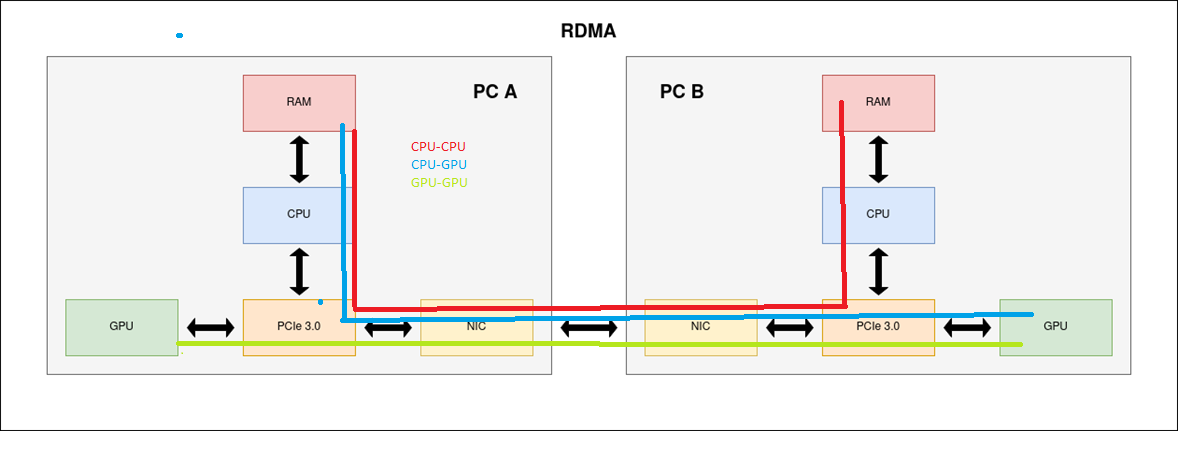
\includegraphics[width = 1\columnwidth]{HLA.png}}
\caption{Flowchart of RDMA for two computers connected with infiniband for RDMA using VERBS.}
\label{HLA}
\end{center}
\end{figure}

\subsection{Verbs}
A high level flowchart of the verbs implementation is found in figure \ref{cpu-cpu2-demo}.
\begin{figure}[H]
\begin{center}
\subfloat[]{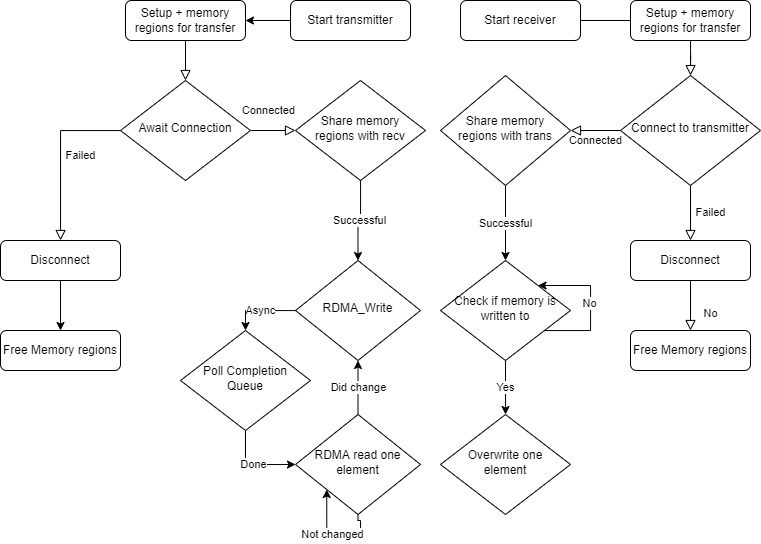
\includegraphics[width = 1\columnwidth]{RDMA_Done.jpg}}
\caption{Flowchart of RDMA for two computers connected with infiniband for RDMA using VERBS.}
\label{cpu-cpu2-demo}
\end{center}
\end{figure}

\subsection{UCX}
Unified Communication X or commonly referred to as UCX is an open-source, production-grade communication framework for data-centric and high-performance applications. UCX can be split into three parts: UCT, UCP and UCS.

\begin{itemize}
   \item \textbf{UCT} acts as a transport layer for the UCX framework. The purpose of UCT is to enable a direct path for network fabrics to access connected devices. To enable efficient resources to the user-space program, UCT relies on kernel drivers such as Verbs, shared memory and CUDA. UCT also defines three levels communication interfaces.
   short (immediate), medium (buffered copy-and-send, bcopy) and large (zero-copy, zcopy) communication operations. The methods are optimized for the size of transfer messages.

   \item \textbf{UCP} implements higher-level protocols that are typically used by message passing interfaces (MPI) and PGAS programming models by using lower-level kernel drivers exposed through the UCT layer. UCP is responsible for initialization of the library, selection of communication methods, message fragmentation, and multi-rail communication. At the time of writing this, UCP handles: Initialization, Remote Memory Access (RMA) communication, Atomic Memory Operations (AMO) and Active Messaging (AM).
   
   \item \textbf{UCS} is a service layer that provides the necessary functionality for implementing portable and efficient utilities.
 \end{itemize}




\subsubsection{Abstraction Layer}
UCX exposes an abstraction level communication layer for the user-space program. The methods include TCP, RDMA, shared memory and network atomic operations.

\subsubsection{UCX-PY}
Using UCX enables rapid development by providing a high-level API at the cost of masking the low-level details, while maintaining high-performance and scalability. Other than C/C++ portability, the project exposes a set of Java and Python bindings. \cite{article_ucx_py}

\noindent\begin{minipage}{.45\textwidth}
Server
\begin{python}
async def server(ep):
    obj = await ep.recv_obj()

lf = ucp.create_listener(server, port) 

while not lf.closed():
    await asyncio.sleep(0.1)
\end{python}

\end{minipage}\hfill
\begin{minipage}{.45\textwidth}
Client
\begin{python}

client = await ucp.create_endpoint(addr, port)


await client.send_obj(obj)
await client.close()
 
 
\end{python}

\end{minipage}

%\begin{python}
%# server
%async def server(ep):
%    obj = await ep.recv_obj()
%
%lf = ucp.create_listener(server, port)  # ucp being UCX-PY 
%
%while not lf.closed():
%    await asyncio.sleep(0.1)
%\end{python}
%
%\begin{python}
%# client
%client = await ucp.create_endpoint(addr, port)  # ucp being UCX-PY
%
%await client.send_obj(obj)
%await client.close()
%\end{python}

\subsubsection{Cython}
UCX-PY bindings were accessed using Cython. Cython is an optimising static compiler for both the Python programming language and the extended Cython programming language (based on Pyrex). Cython allows for C extensions for Python. Cython was used as a superset for the Python language and as a high level bridge for accessing the exposed functions from UCX-PY. This allowed for rapid development without the same performance reduction as the same implementation in pure Python. This speed gain is achieved by no interpretation of the code since the code is compiled beforehand. Furthermore, reading Cython code is similar to Python. Therefore, the reader looking at the source code should be able to understand it, if the reader is familiar with C and Python:

\noindent\begin{minipage}{.45\textwidth}
Cython3 Code
\begin{python}
# cython: language_level=3
from libc.stdio cimport printf

cdef fooPrint(str msg):
    printf("%f\n", msg)
\end{python}

\end{minipage}\hfill
\begin{minipage}{.45\textwidth}
Python3 Code
\begin{python}
#!/usr/bin/env python3
# -*- coding: utf-8 -*-

def fooPrint(msg)
    print(msg)
\end{python}

\end{minipage}

\subsection{UCX Algorithm}

\begin{figure}[H]
\begin{center}
\subfloat[]{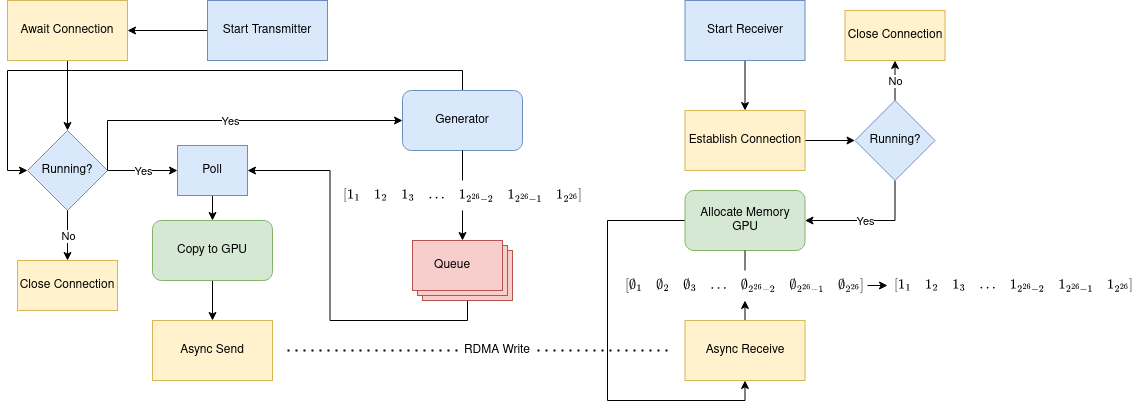
\includegraphics[width = 1\columnwidth]{ucx-algorithm.png}}
\caption{Algorithm flowchart for synthetic\_transfer.}
\label{high-level-ucx}
\end{center}
\end{figure}

The figure \ref{high-level-ucx} visualizing the UCX implementation was developed to process a continuous flow of data, therefore, for the \verb|synthetic\_transfer| data is generated by an arbitrary function on demand. The default is to allocate memory and write an array of $2^{26}$ ones (int8). An abstract pointer to the array is then added to a FIFO queue where another process frees the the first array by performing a send call with the array to a remote recipient. Thereafter, the memory used by the local array is freed. 

The receiving end is same on \verb|synthetic_transfer| and \verb|real_transfer|. The receiving end acts similarly to a server, where the client being the transmitting end.
Therefore, upon start, the receiving end waits for a connection over the UCX protocol


\subsection{Limitations}

\subsubsection{PCIe 3.0}
The motherboards used to conduct the demos were equippped with PCIe 3.0 \cite{article_dell_motherboard} allowing for intra-communication transfer speeds up to 16GB/s (128Gbit/s). 

\subsubsection{Nvidia (Mellanox) ConnectX-6 Dx}
Mellanox Technologies MT2892 Family [ConnectX-6 Dx]
Is a SmartNIC providing secure and fast ethernet connectivity, it is capable of delivering port speeds of 2x12.5/1x25 GB/s (2x100/1x200 Gb/s) with a message rate of 215M messages per second using 16 lanes of PCIe (Gen3 or Gen4) with optional encryption (IPSec/TLS/AES-XTS). Since the motherboards on the demo servers were equipped with PCIe 3.0, the SmartNICs were not able to reach their maximum transfer speeds, but were limited to 16GB/s and since the method incorporated transferring data over multiple ports, we were able to use the two port configuration allowing us to reach less than PCIe 3.0 could deliver, meaning 12.5GB/s

%\cite{article_nvidia_connectx6_dx} Is a SmartNIC providing secure and fast ethernet connectivity, it is capable of delivering port speeds of 2x12.5/1x25 GB/s (2x100/1x200 Gb/s) with a message rate of 215M messages per second using 16 lanes of PCIe (Gen3 or Gen4) with optional encryption (IPSec/TLS/AES-XTS). Since the motherboards on the demo servers were equipped with PCIe 3.0, the SmartNICs were not able to reach their maximum transfer speeds, but were limited to 16GB/s and since the method incorporated transferring data over multiple ports, we were able to use the two port configuration allowing us to reach less than PCIe 3.0 could deliver, meaning 12.5GB/s 

\subsubsection{Layout Topology}
The physical layout of the devices connected to the motherboard contribute to the transfer speeds of the overall configuration, meaning that not all ports on the motherboard are sufficient for fast RDMA transfer. In our configuration, we mounted the SmartNICs to Slot 1 on the motherboard wired as x8 allowing for more power to the cards and higher throughput over 16 lanes. slot 2 and 4 did not allow for sufficient power to the cards, which reduced the transfer-capabilities of the SmartNICs.




\section{Results}

\subsection{UCX}
GPU to GPU memory copy was performed in chunks of data, $2^{26}$ bytes, albeit in a continuous flow. Therefore the transfer-rate was measured as a rolling average over the course of a complete transfer loop, ie. creating an array, await queue pair recipient and finally write to remote memory region. During trials, the synthetic data-transfer rate was measured to be around 5.78GB/s where our theoretical bandwidth per physical Mellanox infiniband wire was 12.5GB/s (100Gbit/s). Therefore achieving a real-time continuous throughput of 46\% of the theoretical maximum.
\subsection{Verbs API}
For all of the tests, CPU to CPU, CPU to GPU and GPU to GPU, RDMA was performed in chunks of $2^{21}$ bytes. This was done 2000 times and an average time was calculated. The throughput for each case can be seen in the following chapter. 



\subsection{CPU-CPU RDMA}
In Figure \ref{cpu-cpu-demo} we can see two cases of when signals are generated with the model of \ref{cpu-cpu-demo}.

\begin{figure}[H]
\begin{center}
\subfloat[]{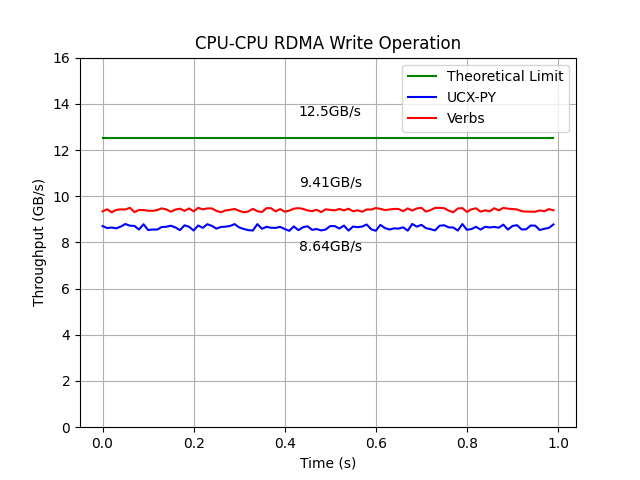
\includegraphics[width = 0.8\columnwidth]{cpu-cpu.png}}
\caption{Transfer throughput results CPU to CPU remote memory copy during 1 second for two different methods: UCX-PY and Verbs. Message size for UCX-PY was $2^{26}$ bytes and Verbs was $2^{21}$ bytes.}
\label{cpu-cpu-demo}
\end{center}
\end{figure}

\subsection{CPU-GPU RDMA}
In Figure \ref{cpu-cpu-demo} we can see two cases of when signals are generated with the model of \ref{cpu-gpu-demo}.

\begin{figure}[H]
\begin{center}
\subfloat[]{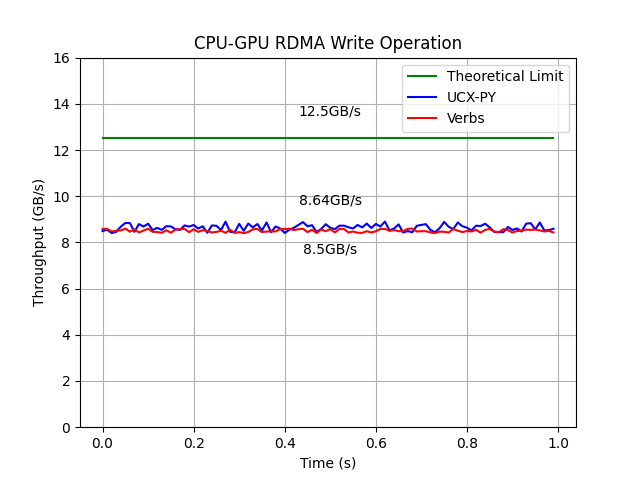
\includegraphics[width = 0.8\columnwidth]{cpu-gpu.png}}
\caption{Transfer throughput results CPU to GPU remote memory copy during 1 second for two different methods: UCX-PY and Verbs. Message size for UCX-PY was $2^{26}$ bytes and Verbs was $2^{21}$ bytes.}
\label{cpu-gpu-demo}
\end{center}
\end{figure}

\subsection{GPU-GPU RDMA}
In Figure \ref{cpu-cpu-demo} we can see two cases of when signals are generated with the model of \ref{gpu-gpu-demo}.


\begin{figure}[H]
\begin{center}
\subfloat[]{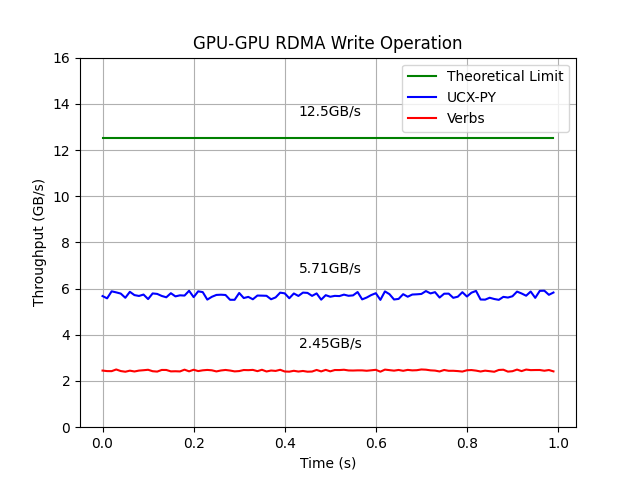
\includegraphics[width = 0.8\columnwidth]{gpu-gpu.png}}
\caption{Transfer throughput results GPU to GPU remote memory copy during 1 second for two different methods: UCX-PY and Verbs. Message size for UCX-PY was $2^{26}$ bytes and Verbs was $2^{21}$ bytes.}
\label{gpu-gpu-demo}
\end{center}
\end{figure}


\pagebreak
\section{Future Work}

\subsection{GPUDirect RDMA}
To successfully use NVIDIAs GPUDirect RDMA technology to copy from a GPU to another GPU with a decent throughput, pinning the GPU memory is essential. This is done by calling functions in kernel space provided by NVIDIA. For instance: \begin{verbatim}
int nvidia_p2p_get_pages(uint64_t p2p_token, uint32_t va_space_token,
                uint64_t virtual_address,
                uint64_t length,
                struct nvidia_p2p_page_table **page_table,
                void (*free_callback)(void *data),
                void *data);

\end{verbatim}
Unfortunately, due to difficulty and time restrictions, this wasn't possible to achieve during this internship. Thus, the Verbs GPU-GPU RDMA was severly underperforming as seen in figure \ref{gpu-gpu-demo}. It is likely required to make your own kernel driver when compiling the rest of your program to achieve this, although that is speculation.

\subsection{PCIe $>3.0$}
This demo utilized motherboards with PCIe 3.0 with a transfer speed limit for 16GB/s, however the Smart NICs are capable of transferring up to 25GB/s which with the newer PCIe 4.0 (2017) is achievable. PCIe 4.0 allow for a combined transfer-speed of all 16 channels a throughput of close to 32GB/s. There are other newer versions such as PCIe 5.0 (2019) with 64GB/s over 16 channels and PCIe 6.0 (2022) with 120GB/s over 16 channels. \cite{article_wikipedia_pcie}

\subsection{RDMA Read}
The \verb|UCX| demo explored the concepts of RDMA Write operations, where one GPU is able to write to a remote peer device without copying through the remote host's CPU. There is however possible to perform a remote read operation, which in conceptual terms would be similar to RDMA write, the difference being who initiates a memory transaction between peer devices. The \verb|UCX| demo found that measuring RDMA Write using UCX-PY operations would be sufficient for the scope of this summer internship, however exploring RDMA Read operations could potentially yield interesting use cases.

RDMA read was used in the Verbs demo handshake to query a memory variable in order to know when the receiver had successfully handled the RDMA write.

\subsection{PeerDirect Async}
There is a another method for accomplishing RDMA between GPU's using the peerdirect async sub-system. This method allows hardware devices such as GPUs to control NICs directly, bypassing the CPU in critical paths. In order to do this, Nvidia created a set of experimental verb calls providing application with abstract description of operation sequences intended to be executed by peer device.

\begin{itemize}
   \item ibv\_exp\_create\_cq
   \subitem ibv\_exp\_peer\_direct\_attr
   \item ibv\_exp\_create\_qp
   \subitem ibv\_exp\_peer\_direct\_attr
   \item ibv\_exp\_peer\_commit\_qp
   \item ibv\_exp\_rollback\_qp
   \item ibv\_exp\_peer\_peek\_cq
   \item ibv\_exp\_peer\_abort\_peek\_cq
 \end{itemize}

    Any verb in the header file \verb|peer_ops.h|

\subsection{Multiple Ports}
Due to time restrictions, the methods used in this demo were single processes who utilized only one physical port on the network card. If the workload was split up among multiple processes over multiple ports, faster transfer-rates would likely be feasible. 

\pagebreak
\bibliographystyle{IEEEtran}
\bibliography{references}

\end{document}